% Options for packages loaded elsewhere
\PassOptionsToPackage{unicode}{hyperref}
\PassOptionsToPackage{hyphens}{url}
\PassOptionsToPackage{dvipsnames,svgnames,x11names}{xcolor}
%
\documentclass[
  letterpaper,
  DIV=11,
  numbers=noendperiod]{scrartcl}

\usepackage{amsmath,amssymb}
\usepackage{iftex}
\ifPDFTeX
  \usepackage[T1]{fontenc}
  \usepackage[utf8]{inputenc}
  \usepackage{textcomp} % provide euro and other symbols
\else % if luatex or xetex
  \usepackage{unicode-math}
  \defaultfontfeatures{Scale=MatchLowercase}
  \defaultfontfeatures[\rmfamily]{Ligatures=TeX,Scale=1}
\fi
\usepackage{lmodern}
\ifPDFTeX\else  
    % xetex/luatex font selection
\fi
% Use upquote if available, for straight quotes in verbatim environments
\IfFileExists{upquote.sty}{\usepackage{upquote}}{}
\IfFileExists{microtype.sty}{% use microtype if available
  \usepackage[]{microtype}
  \UseMicrotypeSet[protrusion]{basicmath} % disable protrusion for tt fonts
}{}
\makeatletter
\@ifundefined{KOMAClassName}{% if non-KOMA class
  \IfFileExists{parskip.sty}{%
    \usepackage{parskip}
  }{% else
    \setlength{\parindent}{0pt}
    \setlength{\parskip}{6pt plus 2pt minus 1pt}}
}{% if KOMA class
  \KOMAoptions{parskip=half}}
\makeatother
\usepackage{xcolor}
\setlength{\emergencystretch}{3em} % prevent overfull lines
\setcounter{secnumdepth}{-\maxdimen} % remove section numbering
% Make \paragraph and \subparagraph free-standing
\makeatletter
\ifx\paragraph\undefined\else
  \let\oldparagraph\paragraph
  \renewcommand{\paragraph}{
    \@ifstar
      \xxxParagraphStar
      \xxxParagraphNoStar
  }
  \newcommand{\xxxParagraphStar}[1]{\oldparagraph*{#1}\mbox{}}
  \newcommand{\xxxParagraphNoStar}[1]{\oldparagraph{#1}\mbox{}}
\fi
\ifx\subparagraph\undefined\else
  \let\oldsubparagraph\subparagraph
  \renewcommand{\subparagraph}{
    \@ifstar
      \xxxSubParagraphStar
      \xxxSubParagraphNoStar
  }
  \newcommand{\xxxSubParagraphStar}[1]{\oldsubparagraph*{#1}\mbox{}}
  \newcommand{\xxxSubParagraphNoStar}[1]{\oldsubparagraph{#1}\mbox{}}
\fi
\makeatother


\providecommand{\tightlist}{%
  \setlength{\itemsep}{0pt}\setlength{\parskip}{0pt}}\usepackage{longtable,booktabs,array}
\usepackage{calc} % for calculating minipage widths
% Correct order of tables after \paragraph or \subparagraph
\usepackage{etoolbox}
\makeatletter
\patchcmd\longtable{\par}{\if@noskipsec\mbox{}\fi\par}{}{}
\makeatother
% Allow footnotes in longtable head/foot
\IfFileExists{footnotehyper.sty}{\usepackage{footnotehyper}}{\usepackage{footnote}}
\makesavenoteenv{longtable}
\usepackage{graphicx}
\makeatletter
\newsavebox\pandoc@box
\newcommand*\pandocbounded[1]{% scales image to fit in text height/width
  \sbox\pandoc@box{#1}%
  \Gscale@div\@tempa{\textheight}{\dimexpr\ht\pandoc@box+\dp\pandoc@box\relax}%
  \Gscale@div\@tempb{\linewidth}{\wd\pandoc@box}%
  \ifdim\@tempb\p@<\@tempa\p@\let\@tempa\@tempb\fi% select the smaller of both
  \ifdim\@tempa\p@<\p@\scalebox{\@tempa}{\usebox\pandoc@box}%
  \else\usebox{\pandoc@box}%
  \fi%
}
% Set default figure placement to htbp
\def\fps@figure{htbp}
\makeatother

\KOMAoption{captions}{tableheading,figureheading}
\makeatletter
\@ifpackageloaded{caption}{}{\usepackage{caption}}
\AtBeginDocument{%
\ifdefined\contentsname
  \renewcommand*\contentsname{Table des matières}
\else
  \newcommand\contentsname{Table des matières}
\fi
\ifdefined\listfigurename
  \renewcommand*\listfigurename{Liste des Figures}
\else
  \newcommand\listfigurename{Liste des Figures}
\fi
\ifdefined\listtablename
  \renewcommand*\listtablename{Liste des Tables}
\else
  \newcommand\listtablename{Liste des Tables}
\fi
\ifdefined\figurename
  \renewcommand*\figurename{Figure}
\else
  \newcommand\figurename{Figure}
\fi
\ifdefined\tablename
  \renewcommand*\tablename{Table}
\else
  \newcommand\tablename{Table}
\fi
}
\@ifpackageloaded{float}{}{\usepackage{float}}
\floatstyle{ruled}
\@ifundefined{c@chapter}{\newfloat{codelisting}{h}{lop}}{\newfloat{codelisting}{h}{lop}[chapter]}
\floatname{codelisting}{Listing}
\newcommand*\listoflistings{\listof{codelisting}{Liste des Listings}}
\makeatother
\makeatletter
\makeatother
\makeatletter
\@ifpackageloaded{caption}{}{\usepackage{caption}}
\@ifpackageloaded{subcaption}{}{\usepackage{subcaption}}
\makeatother

\ifLuaTeX
\usepackage[bidi=basic]{babel}
\else
\usepackage[bidi=default]{babel}
\fi
\babelprovide[main,import]{french}
% get rid of language-specific shorthands (see #6817):
\let\LanguageShortHands\languageshorthands
\def\languageshorthands#1{}
\usepackage{bookmark}

\IfFileExists{xurl.sty}{\usepackage{xurl}}{} % add URL line breaks if available
\urlstyle{same} % disable monospaced font for URLs
\hypersetup{
  pdftitle={La reprise d'emploi est-elle toujours rémunératrice?},
  pdfauthor={Guillaume Allègre; Muriel Pucci},
  pdflang={fr},
  pdfkeywords={Assistance, Prime d'activité, Smic, Gains à l'emploi,
Trappes à inactivité},
  colorlinks=true,
  linkcolor={blue},
  filecolor={Maroon},
  citecolor={Blue},
  urlcolor={Blue},
  pdfcreator={LaTeX via pandoc}}


\title{La reprise d'emploi est-elle toujours rémunératrice?}
\usepackage{etoolbox}
\makeatletter
\providecommand{\subtitle}[1]{% add subtitle to \maketitle
  \apptocmd{\@title}{\par {\large #1 \par}}{}{}
}
\makeatother
\subtitle{Les contradictions des politiques de lutte contre la pauvreté
et comment les surmonter}
\author{Guillaume Allègre \and Muriel Pucci}
\date{2025-09-05}

\begin{document}
\maketitle
\begin{abstract}
Depuis les réformes visant à permettre aux personnes de cumuler
durablement revenus professionnels et prestations sociales, la reprise
d'emploi est toujours rémunératrice. Mais travailler ne permet pas
toujours de sortir de la pauvreté. Cela s'explique notamment par le fait
que le revenu minimum garanti aux personnes d'âge actif est très faible
et maintient la plupart du temps les personnes sans emploi sous le seuil
de grande pauvreté : le travail paie plus que l'assistance, mais les
travailleurs partent de trop bas.
\end{abstract}


\section{Introduction : les objectifs de la lutte contre la pauvreté par
l'emploi}\label{introduction-les-objectifs-de-la-lutte-contre-la-pauvretuxe9-par-lemploi}

Y a-t-il de bonnes raisons de reprendre un emploi payé au salaire
minimum quand on touche des prestations sociales ? Il existe des raisons
non-monétaires de prendre un emploi, notamment en termes d'insertion
sociale. Mais la question posée de façon récurrente est celle des gains
monétaires à l'emploi. On peut ainsi distinguer deux questions :
l'existence des gains, et la sensibilité des travailleurs à ces gains
(l'élasticité de l'offre de travail). Nous nous intéressons ici à la
première de ces questions. Dans un contexte où les aides sociales sont
critiquées pour leur trop grande générosité et où les politiques de tout
bord insistent sur la valeur travail, le travail doit payer et bien plus
que l'assistance.

La stratégie nationale de prévention et de lutte contre la pauvreté
(SNPLP), publiée en 2018 permet de préciser les objectifs de la
politique sociale en termes de lutte contre la pauvreté et de gains à
l'emploi. Elle prévoit la création d'un revenu universel d'activité
(RUA) permettant à chacun de vivre décemment et d'accéder plus
rapidement à l'emploi. Plus précisément, on peut dégager les trois
objectifs suivant de la stratégie :

\begin{enumerate}
\def\labelenumi{\arabic{enumi}.}
\tightlist
\item
  ``faire en sorte que le travail paye et qu'il paye de la même façon
  dans tous les cas'' ;
\item
  ``engager une poltique déterminée de sortie de la pauvreté par le
  travail''
\item
  ``garantir un souvien financier aux ménages modestes''
\end{enumerate}

Puisque le travail doit faire sortir de la pauvreté, la stratégie admet
implicitiment que les personnes sans emploi puissent être pauvres. Mais
il ne faut pas que leurs privations soient trop sévères, en particulier
lorsqu'elles ont des enfants. en revanche, la pauvreté en emploi est
perçue comme une anomalie que les politiques publiques doivent corriger
(Allègre, 2024).

Ce document évalue le systèm actuel à l'aune de ces trois objectifs puis
discute des contradiction su système social et des pistes de réforme.

\begin{figure}[H]

\caption{\label{fig-ndv}Niveau de vie (en euros par uc) du revenu
d'assistance et des allocations logement selon la configuration
familiale, pour un foyer sans revenu primaire}

\centering{

\pandocbounded{\includegraphics[keepaspectratio]{PB_GainEmploi_files/figure-pdf/fig-ndv-1.png}}

}

\end{figure}%

La reprise d'emploi est-elle rémunératrice ? Pour répondre à la question
de façon concrète, nous raisonnons sur cas-type. Il s'agit d'illustrer
les gains à la reprise d'emploi en prenant des exemples-type de
situations de travail, de configuration familiale, de logement (pour
calculer les allocations-logement) et éventuellement de modes de gardes
des jeunes enfants. Dans ces situations, les gains à la reprise
d'emploi, proviennent des salaires nets perçus et de la Prime
d'activité. Les ``coûts'' proviennent de l'augmentation de l'impôt sur
le revenu et de la baisse des prestations sociales (RSA, Allocations
logement, prestations familiales\ldots). La variable d'intérêt est le
revenu disponible qui est calculé au niveau du ménage et ne tient pas
compte de la répartition interindividuelle des revenus au sein des
couples. L'analyse porte sur la variation du revenu disponible
lorsqu'une personne passe de l'inactivité à l'emploi ou augmente sa
durée de travail sans tenir compte des coûts associés en termes de
transport ou d'habillement.

\begin{longtable}[]{@{}
  >{\raggedright\arraybackslash}p{(\linewidth - 0\tabcolsep) * \real{1.0010}}@{}}
\caption[Le cas-type général commenté dans le texte est celui d'un
ménage éligible, sous condition de ressources, au RSA (l'individu
référent est âgé entre 25 et 64 ans) et aux allocations logement (le
ménage est locataire du parc privé). Pour les ménages non éligibles à
ces prestations, les prestations sociales sont bien plus faibles, et les
gains à la reprise d'emploi sont donc par construction plus importants.
Pour les ménages avec enfants, nous supposons dans le cas général que
les enfants sont d'âge scolaire (5, 8 ou 10 ans) mais la situation des
familles ayant un enfant en bas âge qui nécessite un mode de garde est
étudiée section 1.4.]{Le cas-type général commenté dans le texte est
celui d'un ménage éligible, sous condition de ressources, au RSA
(l'individu référent est âgé entre 25 et 64 ans) et aux allocations
logement\footnote{On suppose que le ménage est locataire en zone 2 des
  aides au logement (ville moyenne) pour un loyer compris entre 1 et 2,5
  fois le loyer plafond.} (le ménage est locataire du parc privé). Pour
les ménages non éligibles à ces prestations, les prestations sociales
sont bien plus faibles, et les gains à la reprise d'emploi sont donc par
construction plus importants. Pour les ménages avec enfants, nous
supposons dans le cas général que les enfants sont d'âge scolaire (5, 8
ou 10 ans) mais la situation des familles ayant un enfant en bas âge qui
nécessite un mode de garde est étudiée section 1.4.}\tabularnewline
\toprule\noalign{}
\endfirsthead
\endhead
\bottomrule\noalign{}
\endlastfoot
\begin{minipage}[t]{\linewidth}\raggedright
\textbf{Définition : taux effectif de prélèvement et taux effectif de
gain à l'emploi}

\begin{quote}
Outre la variation de revenu disponible du ménage, il est également
possible de calculer un taux effectif de prélèvement (TEP) qui
correspond à la baisse des transferts sociaux (nets d'impôt) par euro
supplémentaire de revenu professionnel. Si, lorsque le revenu d'activité
augmente de 1000 euros, les transferts sociaux nets baissent de 400
euros on dira que le TEP est de 40\%. Dans ce cas, le revenu disponible
augmente de 600 euros.
\[TEP=\frac{\text{-Variation des transferts sociaux nets}}{\text{Variation du revenu professionnel}}=1-\frac{\text{Variation du revenu disponible}}{\text{Variation du revenu professionnel}}\]
On peut définir le taux effectif de gain à l'emploi (TEG) comme la part
de l'augmentation du revenu professionnel qui se traduit en augmentation
du revenu disponible. Si lorsque le revenu d'activité augmente de 1000
euros, le revenu disponible augmente de 600 euros, on dira que le TEG
est de 60\%.
\[TEG=\frac{\text{Variation du revenu disponible}}{\text{Variation du revenu professionnel}}\]
\end{quote}
\end{minipage} \\
\end{longtable}

Trois situations de reprise d'emploi sont analysées : le mi-temps au
Smic horaire (699 euros mensuels), le temps-plein au Smic horaire (1399
euros mensuels) et le temps plein à 1,5 Smic horaire (2098 euros
mensuels). Pour les couples, ces reprises d'emploi sont analysées dans
le cas d'un conjoint inactif sans revenu, d'un conjoint chômeur (avec un
montant d'allocation chômage égal au Smic mensuel) et d'un conjoint en
emploi à temps-plein gagnant le Smic ou 1,5 fois le Smic. L'analyse
n'est pas genrée, mais dans les couples, ce sont le plus souvent les
femmes qui prennent des emplois à mi-temps, à la fois parce que le
partage des tâches reste très inégalitaire et parce qu'elles ont des
emplois dans des secteurs où elles plus sont plus susceptibles d'être en
temps-partiel subi (ref). L'analyse est descriptive et ne présume pas
que les ménages ou individus ont le choix entre les différents horaires
de travail ou taux de salaire.

L'approche en termes de revenus disponibles, ou niveaux de vie, ne tient
compte ni des différences de coûts de la vie induits par le fait de
travailler plutôt qu'être au foyer, en particulier dans les ménages avec
enfants, ou lorsque le trajet domicile-travail est coûteux, ni des aides
locales sous conditions de ressources (tarification de la cantine
scolaire). Elle ne tient pas compte non plus des avantages économiques
liés à l'emploi qu'ils soient immédiats (tickets restaurant, prise en
charge des cartes de transport) ou différés droits ouverts en termes de
chômage ou retraite).~L'approche néglige également le fait que les
personnes peuvent valoriser différemment les salaires et les prestations
sociales. Cette approche est simplificatrice mais elle est cohérente
avec la mesure du niveau de vie et de la pauvreté monétaire.

L'approche par cas-type est critiquable dans la mesure où elle ne
représente pas la diversité des situations individuelles. Par
construction, elle renseigne, de façon synthétique, plutôt sur les
caractéristiques du système social et fiscal que sur celles des ménages
concernés. L'analyse est descriptive et ne présuppose pas que les
individus ont le choix entre les différents horaires de travail ou taux
de salaire

\subsection{1. La reprise d'emploi est toujours rémunératrice, mais pas
toujours de façon
homogène}\label{la-reprise-demploi-est-toujours-ruxe9munuxe9ratrice-mais-pas-toujours-de-fauxe7on-homoguxe8ne}

\subsection{1.1. Des reprises d'emploi
rémunératrices}\label{des-reprises-demploi-ruxe9munuxe9ratrices}

Dans les cas types étudiés, le système socio-fiscal actuel garantit que
la reprise d'emploi est toujours rémunératrice, mais pas nécessairement
toujours dans les mêmes proportions.

Le cas d'une personne seule illustre la façon dont le système
socio-fiscal assure que le travail paie mieux que l'assistance, même
pour de petites durées de travail. Sans revenus d'activité, cette
personne peut percevoir 851 euros de prestations sociales (559 euros de
RSA et 292 euros d'allocations logement), ce qui est juste en dessous du
seuil de grande pauvreté à 40\% du niveau de vie médian\footnote{Son
  niveau de vie équivaut à 39\% du niveau de vie médian.}.

\begin{figure}[H]

\caption{\label{fig-C1A0E}Revenu disponible d'une personne seule selon
son revenu professionnel}

\centering{

\pandocbounded{\includegraphics[keepaspectratio]{PB_GainEmploi_files/figure-pdf/fig-C1A0E-1.png}}

}

\end{figure}%

Si cette personne reprend un emploi rémunéré au Smic, son revenu
disponible augmente que l'emploi soit à temps partiel ou à temps plein,
en dépit de la baisse du montant de prestations sociales. Avec un emploi
à mi-temps, le revenu disponible est de 1 191 euros et le taux effectif
de gain à l'emploi (TEG) est de 48,6\% (soit un taux effectif de
prélèvement de 51,4\%), ce qui veut dire que les ménages gardent en
revenu disponible seulement 340 euros sur les 699 euros de salaire
reçus. Cela s'explique par la baisse du montant d'aides au logement et
par la perte du RSA, compensée en partie seulement par la prime
d'activité. Avec un emploi à temps-plein, le revenu disponible double
quasiment (+94\%) et atteint 1656 euros (soit une hausse de 805 euros)
avec un TEG de 57,5\%, plus élevé que pour une emploi à mi-temps en
dépit de la perte des aides au logement. Si l'emploi à temps plein est
rémunéré à 1,5 Smic, le niveau de vie atteint 2 016 euros (hausse de 1
165 euros) et le TEG est de 55,5\% car relativement à la situation
d'inactivité, le travailleur perd à la fois le RSA et les aides au
logement mais n'a pas droit à la prime d'activité.

Pour un couple avec deux enfants (âgés de 5 et 8 ans) initialement sans
revenu et dont un des conjoints reprend un emploi à plein-temps, le gain
de revenu disponible en euros est de 845 euros, soit un gain très proche
de celui du célibataire sans enfant, et par conséquent un TEG également
similaire (60,4\% contre 57,5\% pour une personne seule). Si le gain en
euro est similaire, ce couple a un revenu disponible plus important en
situation d'inactivité (1 652 euros) et le gain relatif est donc moindre
(+51\%). De plus, ce couple comporte davantage d'unités de consommation
que le célibataire et pour une augmentation équivalente du revenu
disponible, le gain en niveau de vie est deux fois plus faible que pour
le célibataire sans enfant (402 euros par UC). Comparativement à une
personne seule, le couple monoactif continue à percevoir du RSA avec un
emploi à mi-temps, et il reste éligible aux aides au logement et à la
prime d'activité avec un emploi rémunéré à 1,5 Smic. Mais alors que la
personne seule franchit largement le seuil de pauvreté monétaire avec un
emploi au Smic, le couple monoactif l'atteint tout juste avec un emploi
à 1,5 Smic.

\begin{figure}[H]

\caption{\label{fig-C2A2ECI}Revenu disponible d'un couple avec 2 enfants
selon le revenu professionnel, conjoint inactif}

\centering{

\pandocbounded{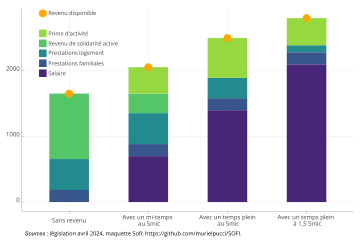
\includegraphics[keepaspectratio]{PB_GainEmploi_files/figure-pdf/fig-C2A2ECI-1.png}}

}

\end{figure}%

\begin{longtable}[]{@{}
  >{\raggedright\arraybackslash}p{(\linewidth - 0\tabcolsep) * \real{1.0011}}@{}}
\toprule\noalign{}
\endhead
\bottomrule\noalign{}
\endlastfoot
\textbf{Définition : niveau de vie}

Le niveau de vie d'un ménage est un indicateur conçu pour comparer les
revenus disponibles de ménages de configuration différentes en tenant
compte des économies d'échelle liées à la vie commune et des dépenses
pour les enfants. Il est obtenu en divisant le revenu disponible de
l'ensemble du ménage par un nombre d'unités de consommation. En France
et en Europe, les unités de consommation sont calculées par l'INSEE et
Eurostat selon l'échelle d'équivalence dite de l'OCDE modifiée qui
attribue 1 UC au premier adulte du ménage, 0,5 UC aux autres personnes
de 14 ans ou plus et 0,3 UC aux enfants de moins de 14 ans (car
considérés comme ayant moins de besoins). Selon cette convention, le
niveau de vie est considéré comme identique pour une personne seule avec
un revenu disponible de 2~000 euros, un couple sans enfant qui dispose
3000 euros (1,5x2000), ou un couple avec un enfants de 10 ans qui
dispose de 3~600 euros (1,8x2000). \\
\end{longtable}

La situation est un peu différente pour une personne en couple avec deux
enfants si le conjoint est actif en emploi, rémunéré sur la base d'un
Smic mensuel. Dans ce cas, le revenu disponible du couple avec deux
enfants est de 2 497 euros en cas de monoactivité, ce qui le situe
au-dessus du seuil de grande pauvreté, et la reprise d'emploi permet de
franchir le seuil de pauvreté à 60~\% même avec un emploi à mi-temps. La
reprise d'emploi à temps plein au Smic est plus rémunératrice que pour
une personne seule ou un couple monoactif avec deux enfants car la
dégressivité des aides est moindre. Cela s'explique par le fait que le
couple ne perçoit pas le RSA avant la reprise d'emploi et que celle-ci
se traduit uniquement par une baisse des aides au logement du montant de
prime d'activité du couple. Le gain associé au second emploi dans le
couple est alors de 911 € ce qui correspond à un TEG de 65\%.

\begin{figure}[H]

\caption{\label{fig-C2A2EC1S}Revenu disponible couple 2 enfants,
conjoint au Smic à plein-temps}

\centering{

\pandocbounded{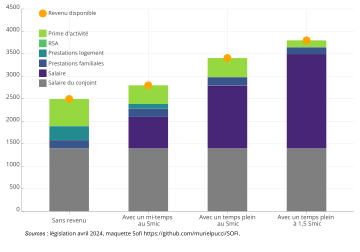
\includegraphics[keepaspectratio]{PB_GainEmploi_files/figure-pdf/fig-C2A2EC1S-1.png}}

}

\end{figure}%

Les gains à l'emploi sont encore plus importants si le revenu du
conjoint, pour un même montant égal au Smic à temps plein, est une
allocation chômage. Dans ce cas, lorsque le travailleur étudié n'a aucun
revenu, le couple monoactif a un revenu disponible plus faible que dans
le cas précédent (1~891~euros contre 2~497 euros) car contrairement au
salaire, l'allocation chômage du conjoint n'ouvre pas droit à la prime
d'activité. La reprise d'emploi a donc un effet plus faible sur le
montant de prestations perçues et le gain à l'emploi pour un Smic à
temps plein est de 1~090 euros, ce qui correspond à un TEG de 78\%. Le
taux effectif de gain est également élevé pour un emploi a mi-temps
(71\%) ou à temps plein avec un salaire de 1,5 Smic (83\%).

\begin{figure}[H]

\caption{\label{fig-C2A2ECCH}Revenu disponible d'un couple avec deux
enfants selon le revenu professionnel, conjoint au chômage (ARE=1 smic)}

\centering{

\pandocbounded{\includegraphics[keepaspectratio]{PB_GainEmploi_files/figure-pdf/fig-C2A2ECCH-1.png}}

}

\end{figure}%

Le système social et fiscal remplit donc l'objectif qui lui a été fixé
depuis la mise en place du RSA en 2009~: rendre le travail plus
rémunérateur que l'assistance, de façon pérenne et pour toutes les
reprises d'emploi. Toutefois les gains effectifs à la reprise d'emploi
sont loin d'être homogènes.

\begin{figure}[H]

\caption{\label{fig-TGE}Taux effectif de gain à l'emploi pour une
reprise d'emploi au Smic à temps-plein, selon la configuration
familiale}

\centering{

\pandocbounded{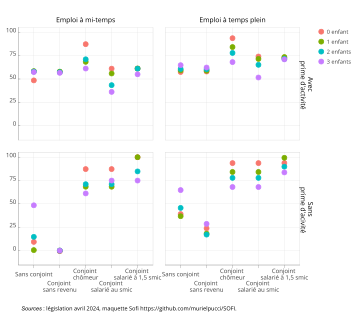
\includegraphics[keepaspectratio]{PB_GainEmploi_files/figure-pdf/fig-TGE-1.png}}

}

\end{figure}%

Pour les cas que nous avons étudiés, le taux effectif de gain pour le
passage de l'inactivité à un emploi à temps plein rémunéré au Smic varie
de 58\% à 65\% pour une personne seule selon le nombre d'enfants à
charge et de 52\% à 94\% pour une personne vivant en couple selon le
montant du revenu du conjoint, sa nature, et le nombre d'enfants à
charge. Le TEG le plus faible est alors obtenu avec 3 enfants lorsque le
conjoint est salarié au Smic car la reprise d'emploi réduit à la fois
les montants de prestations familiales (-97~€), d'aides au logement
(-349~€) et de prime d'activité (-231~€). Le gain le plus élevé est
obtenu avec un conjoint chômeur et aucun enfant à charge car le couple
ne bénéficie initialement que des aides au logement (89€) et n'a donc
que cela à perdre.

Le taux effectif de gain pour le passage de l'inactivité à un emploi à
mi-temps au Smic est plus faible. Il varie de 48\% à 58\% pour une
personne seule selon le nombre d'enfants à charge et de 36\% à 87\% pour
une personne vivant en couple selon le montant du revenu du conjoint, sa
nature, et le nombre d'enfants à charge. Comme pour l'emploi à temps
plein, le TEG le plus faible est alors obtenu avec 3 enfants lorsque le
conjoint est salarié au Smic et le plus élevé est obtenu avec un
conjoint chômeur et aucun enfant à charge.

\begin{figure}[H]

\caption{\label{fig-TGE2}Taux effectif de gain à l'emploi pour une
reprise d'emploi au Smic à mi-temps selon la configuration familiale}

\centering{

\pandocbounded{\includegraphics[keepaspectratio]{PB_GainEmploi_files/figure-pdf/fig-TGE2-1.png}}

}

\end{figure}%

\begin{longtable}[]{@{}
  >{\raggedright\arraybackslash}p{(\linewidth - 0\tabcolsep) * \real{1.0006}}@{}}
\toprule\noalign{}
\endhead
\bottomrule\noalign{}
\endlastfoot
\textbf{Encadré : La prime d'activité}

Depuis le 1er janvier 2016, la prime d'activité a remplacé le RSA
activité et la prime pour l'emploi. Comme les instruments qu'elle
remplace, la prime d'activité vise deux objectifs : soutenir l'offre de
travail grâce à des incitations financières accrues et compléter les
revenus des travailleurs ayant des revenus modestes. La prime pour
l'emploi et le RSA activité ont été critiqués pour leur faible
efficacité (Cahuc, 2002 ; Domingo et Pucci 2014). Individualisée, la
prime pour l'emploi versait de faibles montants à de nombreux
bénéficiaires : trop faible pour être véritablement incitative, elle
bénéficiait de plus à des ménages à niveau de vie intermédiaire et non
aux plus modestes. Le RSA activité tenait compte de la composition et du
revenu du ménage : il était davantage ciblé sur les travailleurs pauvres
et créait des incitations à la reprise d'emploi substantielles et
contemporaines. Néanmoins, son efficacité était minée par un non-recours
élevé (68 \%, voir Domingo et Pucci, 2014). La prime d'activité est
proche dans son fonctionnement du RSA activité : familialisée, versée
mensuellement, après une déclaration trimestrielle de revenus, elle
cible les travailleurs aux revenus modestes et amplifie les incitations
à la reprise d'emploi par le mécanisme des bonus individuels . Elle est
en outre clairement identifiée comme une prestation à destination des
personnes exerçant une activité, ce qui évite qu'elle apparaisse
stigmatisante aux yeux de ceux qui la perçoivent. Par conséquent, le
non-recours est probablement bien plus faible que celui qui était
observé pour le RSA activité, bien qu'il n'y ait pas d'estimation
précise (DREES, 2022). La formule de calcul de la prime d'activité est
la suivante :

\emph{Prime d'activité du foyer =}

\emph{Montant forfaitaire (fonction de la situation familiale)}

\emph{+ bonus d'activité individuels}

\emph{- forfait logement + prestations familiales + minima sociaux}

\emph{- 39 \% des revenus professionnels}

\emph{- 100 \% des revenus non professionnels}

Le montant de la prime d'activité versée au foyer est nul si le résultat
de ce calcul est inférieur à 15 euros. Si elle permet de garantir des
gains entre inactivité et revenus du travail dans presque toutes les
configurations, la prime d'activité a des limites. Par rapport à une
hausse du Smic, c'est une prestation sociale et pas un salaire donnant
des droits sociaux (chômage, retraites). Comme la formule le montre, les
revenus non professionnels du foyer sont déduits à 100\%. Par
conséquent, si dans un couple biactif l'un des conjoints perd son emploi
pour du chômage indemnisé, non seulement il perd son bonus d'activité
individuel, mais son allocation chômage est déduite intégralement ce qui
peut annuler la prime d'activité pour son conjoint resté en emploi. En
pratique, dans la plupart des cas, les ménages incluant un chômeur
indemnisé (ou un retraité) ne touchent pas de prime d'activité. Enfin,
visant à lutter contre les trappes à inactivité, les compléments de
revenus pour travailleurs pauvres sont critiqués en raison des trappes à
bas salaire qu'ils engendrent. En matière d'incitations, ces compléments
ciblés dégressifs ne peuvent que creuser une nouvelle trappe pour
reboucher l'autre : si la prime d'activité augmente l'écart entre emploi
et chômage ou inactivité, elle ne peut que réduire le gain de niveau de
vie induit par une hausse de salaire. \\
\end{longtable}

\subsection{1.3 La nouvelle courbe des gains marginaux à
l'emploi}\label{la-nouvelle-courbe-des-gains-marginaux-uxe0-lemploi}

Le graphique suivant décrit les gains marginaux pour quatre
configurations familiales à six niveaux de revenu (de 0,5 à 2 Smic
mensuel à temps-plein). Le gain marginal à l'emploi est ce qui reste au
foyer lorsque l'individu analysé augmente ses revenus du travail de 100
euros. Les cas-types analysés sont ceux de la personne isolée sans
enfant, du couple monoactif avec deux enfants, du couple biactif sans
enfant ou avec deux enfants, en supposant que le conjoint ou la
conjointe est employée au Smic à plein-temps.

Le graphique montre que sur la plage de revenus considérée, les gains
marginaux à l'emploi sont plus élevés en bas de l'échelle de revenus et
en haut\ldots{} et plus faible au milieu, autour de 1 à 1,2 Smic. Cela
veut dire à l'inverse que les taux marginaux effectifs de prélèvement
sont en U inversé\ldots{} La courbe actuelle suit ainsi le profil opposé
de la courbe ``optimale'' en U des taux marginaux, telle que décrite par
Diamond (1998) ou Saez (2001). Selon ces auteurs, les taux marginaux
effectifs de prélèvement les plus bas devraient s'appliquer au milieu de
l'échelle de revenus, là où les individus sont les plus nombreux. C'est
d'ailleurs ce que faisaient les systèmes socio-fiscaux avant les
réformes dans années 2000.

Avec les réformes visant à rendre le travail payant, les plus faibles
gains à l'emploi se sont déplacés au niveau du Smic ou juste au-dessus
du Smic. Certains pourraient dire que les ``trappes à inactivité'' se
sont transformées en ``trappes à bas salaires'' mais ces expressions ne
sont pas appropriées puisqu'elles impliquent que les travailleurs
répondent à ces plus faibles incitations. Or, il est difficile de
trouver des études confirmant ces effets sur l'offre de travail en
pratique. Selon le rapport Bozio-Wasmer (2024) sur les politiques
d'exonérations sociales (ciblées autour du Smic à temps-plein), si les
effets théoriques des exonérations et des primes d'activité dégressives
sont soulignés régulièrement par les économistes, ``la démonstration
empirique de l'existence de trappes à bas salaire est néanmoins
délicate'', la littérature disponible en France offrant des évidences
empiriques limitées.

Le débat sans fin sur les trappes plaiderait pour une égalisation des
gains marginaux à l'emploi (ou des taux marginaux de prélèvement) selon
le niveau de revenu. Si l'argument le plus convaincant pour des gains à
l'emploi élevés est celui de la rémunération du mérite, alors il n'y a
pas de raison fondamentale pour que les gains marginaux ou taux
marginaux de prélèvement fluctuent dans le bas de l'échelle des revenus.

\begin{figure}[H]

\caption{\label{fig-gainsmarginaux}Gain marginaux effectifs pour une
augmentation de 100 euros du revenu d'activité, selon la configuration
familiale et le niveau de revenu initial}

\centering{

\pandocbounded{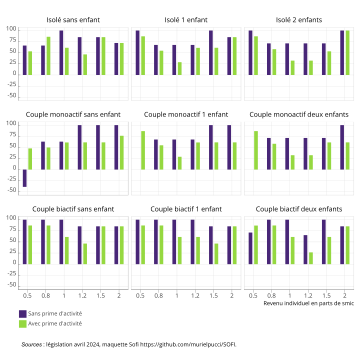
\includegraphics[keepaspectratio]{PB_GainEmploi_files/figure-pdf/fig-gainsmarginaux-1.png}}

}

\end{figure}%

\subsection{1.4 Que change la prise en compte des coûts de garde des
jeunes enfants
?}\label{que-change-la-prise-en-compte-des-couxfbts-de-garde-des-jeunes-enfants}

Pour illustrer les effets du coût de la garde sur les gains à l'emploi
des familles avec de jeunes enfants, nous étudions ici deux cas-types de
familles avec un enfant de 1 an : une mère isolée et celui un couple
dans lequel le conjoint travaille à temps-plein rémunéré au Smic. On
suppose que lorsque la mère travaille, l'enfant est gardé par une
assistante maternelle, la garde onéreuse la plus courante, au prorata du
temps de travail de la mère.

Comme le montre le graphique suivant, le coût net de la garde est
relativement modéré et représente 300 euros maximum, soit environ 10\%
du revenu disponible lorsque les deux conjoints sont au Smic à
temps-plein. Néanmoins on peut également voir que le coût net de la
garde augmente rapidement entre le mi-temps et le temps-plein (il passe
de 50 à 300 euros). Par conséquent, les incitations à passer du mi-temps
au temps-plein deviennent faibles dans ces cas.

\begin{figure}[H]

\caption{Revenu disponible après coût de garde selon le revenu
professionnel et la configuration familiale}

{\centering \pandocbounded{\includegraphics[keepaspectratio]{PB_GainEmploi_files/figure-pdf/fig_gard-1.png}}

}

\end{figure}%

\begin{figure}[H]

\caption{Revenu disponible après coût de garde selon le revenu
professionnel et la configuration familiale}

{\centering \pandocbounded{\includegraphics[keepaspectratio]{PB_GainEmploi_files/figure-pdf/fig_gard-2.png}}

}

\end{figure}%

\section{2. L'emploi ne protège pas toujours de la
pauvreté}\label{lemploi-ne-protuxe8ge-pas-toujours-de-la-pauvretuxe9}

Si l'emploi est toujours rémunérateur (1), il ne protège pas toujours de
la pauvreté monétaire. Ceci apparaît clairement sur cas types mais peut
se voir également par l'existence d'une pauvreté monétaire en emploi,
même pour des bénéficiaires de la prime d'activité\footnote{Si la prime
  d'activité permet à certains foyers de franchir le seuil de pauvreté
  monétaire, l'analyse par cas types montre que certains foyers à bas
  salaire n'y sont pas éligibles. S'y ajoutent ceux qui ne recourent pas
  à cette prestation bien que leur niveau de vie soit inférieur au seuil
  de pauvreté monétaire.}. En 2022, selon l'INSEE le taux de pauvreté
sur l'ensemble de la population était de 14,4\%. et celui des personnes
en emploi de 7,8 \%. Mais en se limitant aux personnes en emploi vivant
dans un ménage allocataire de la prime d'activité, ce taux atteint 15,2
\%. L'emploi réduit ainsi beaucoup le risque de pauvreté monétaire mais
ne l'annule pas : sur les 9,1 millions de personnes vivant sous le seuil
de pauvreté monétaire, 2~millions sont en emploi (INSEE).

\begin{longtable}[]{@{}
  >{\raggedright\arraybackslash}p{(\linewidth - 0\tabcolsep) * \real{1.0009}}@{}}
\toprule\noalign{}
\endhead
\bottomrule\noalign{}
\endlastfoot
\textbf{Définition : la pauvreté monétaire et les privations matérielles
et sociales}

D'après la statistique publique (INSEE, Eurostat), un individu est
pauvre d'un point de vue monétaire si le niveau de vie du ménage auquel
il appartient est inférieur à 60\% du niveau de vie médian. La pauvreté
monétaire est ainsi un concept relatif : si le niveau de vie de tous les
ménages augmente de 10\%, le taux de pauvreté monétaire restera
inchangé. Par convention, le seuil de pauvreté monétaire est le même
dans tout le pays, mais il varie au sein de l'Union Européenne d'un pays
à l'autre. La pauvreté monétaire est donc définie uniquement par les
revenus. La seule prise en compte des différences de besoins se fait par
l'échelle d'équivalence qui définit le nombre d'unités de consommation
du ménage selon sa composition. Le niveau de vie ne prend donc pas en
compte le coût du logement ni les besoins différenciés en transport,
logement ou chauffage selon le lieu de vie. Le dernier seuil de pauvreté
monétaire publié par l'Insee est de 1~216 euros par UC pour l'année
2022. Pour le comparer aux montants des prestations en 2024, nous avons
appliqué à ce seuil l'inflation observée entre 2022 et juillet 2024, ce
qui amène à un seuil de 1~309 euros par UC.

Le taux de privation matérielle et sociale est un indicateur social
utilisé dans l'union européenne, défini comme la part de personnes ne
pouvant pas couvrir les dépenses liées à au moins cinq éléments de la
vie courante sur treize considérés comme souhaitables, voire
nécessaires, pour avoir un niveau de vie acceptable (Guio et al, 2017).

L'intensité de la pauvreté mesure l'écart relatif entre le niveau de vie
médian de la population pauvre et le seuil de pauvreté. \\
\end{longtable}

Le niveau de vie d'un célibataire sans enfant sans revenus d'activité et
recourant à toutes les prestations est de 851 euros par uc ce qui est
inférieur de 35\% au seuil de pauvreté monétaire : son intensité de
pauvreté est donc de 35\%. Un emploi à mi-temps au Smic ne lui permet
pas de franchir le seuil de pauvreté (intensité de 9\%). Le célibataire
sans enfant franchit le seuil de pauvreté monétaire avec un Smic à plein
temps même s'il ne recourt pas à la prime d'activité et son niveau de
vie atteint 126\% du seuil s'il y recourt. En revanche, un emploi à
mi-temps ne permet pas se sortir de la pauvreté même si la prime
d'activité en réduit l'intensité (de 30\% avant prime à 9\% après).

Une personne isolée avec enfant(s) en emploi à plein-temps au Smic est
au-dessus du seuil de pauvreté monétaire, qu'elle ait un enfant (125\%)
du seuil), deux enfants (119\%), ou trois enfants (124\%) et elle le
serait même sans la prime d'activité. Le système socio-fiscal permet
donc bien aux parents isolés de sortir de la pauvreté lorsqu'elles
travaillent au Smic à temps plein et la prime d'activité leur permet de
dépasser largement le seuil. La prime d'activité permet même aux parents
isolés d'atteindre\footnote{Avec 2 enfants, le niveau de vie prime
  d'activité comprise atteint 98\% su seuil de pauvreté. Il est égale au
  seuil avec avec enfant et le dépasse de 4\% acvec trois enfants.} le
seuil de pauvreté avec un emploi à mi-temps au Smic.

Les revenus d'un couple monoactif dans lequel l'un des conjoints
travaille au Smic à plein-temps, et l'autre conjoint est sans revenu ;
permettent tout juste d'atteindre le seuil de pauvreté si le couple n'a
pas d'enfant à condition que celui-ci recoure à la prime d'activité
(sinon le niveau de vie atteint seulement 76\% du seuil de pauvreté). A
ce niveau de revenus, le système social ne compense pas entièrement la
charge des enfants, et le niveau de vie des couples monoactifs avec
enfants est légèrement plus faible quand ils ont des enfants que quand
ils n'en ont pas. L'intensité de la pauvreté monétaire est alors de 7\%
s'ils ont un enfant, 9\% avec deux enfants, et 5\% avec trois enfants.

Les couples biactifs avec deux emploi au Smic à temps-plein ont un
revenu disponible avant prime d'activité supérieur au seuil de pauvreté
et dépassent largement ce seuil avec la prime. Qu'ils recourent ou non à
la prime d'activité, le système socio-fiscal ne compense que
partiellement la charge des enfants telle qu'elle est appréhendée par
les unités de consommation. Un couple biactif au Smic recourant à la
prime d'activité a ainsi un niveau de vie équivalent à 153\% du seuil de
pauvreté s'il n'a pas d'enfant, 135\% du seuil de pauvreté s'il en a un,
124\% avec deux enfants et 117\% avec trois (contre 142\%, 119\%, 108\%
et 110\% respectivement s'il n'y recourt pas).

\begin{figure}[H]

\caption{\label{fig-pauvreté}taux de pauvreté et taux de privation
matérielle selon la tranche de revenu salarial et la configuration
familiale}

\centering{

\pandocbounded{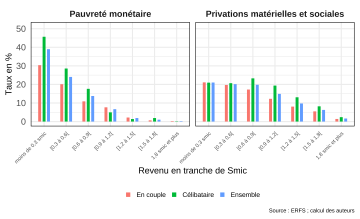
\includegraphics[keepaspectratio]{PB_GainEmploi_files/figure-pdf/fig-pauvreté-1.png}}

}

\end{figure}%

Les graphiques représentent les taux de pauvreté monétaire (gauche) et
de privation matérielle et sociale (droite) des individus selon leur
revenu salarial mensuel (en tranche de Smic) et leur situation conjugale
(en couple ou célibataire). Le taux de pauvreté monétaire baisse
nettement lorsque les revenus salariaux augmentent. Cette baisse de la
pauvreté est liée directement à l'augmentation des salaires (composantes
du niveau de vie), mais aussi à des caractéristiques plus favorables.

Le taux de privation matérielle et sociale baisse également lorsque le
salaire augmente, mais la baisse est plus franche seulement à partir du
Smic. Cela suggère qu'il existe un coût à travailler de faibles nombre
d'heures et que ce coût compense la hausse du salaire net et du revenu
disponible. Ce coût peut être lié au transport ou à la garde d'enfants.

Si l'hypothèse du coût pour les emplois à temps-partiel est juste, il
existe deux réponses possibles en termes de politiques publiques :
inciter de façon monétaire les individus pour qu'ils acceptent ces
emplois ou favoriser une norme de plein-emploi. Avant d'exposer nos
recommandations (section 4), on peut noter qu'inciter au temps-partiel
ou très-partiel, que ce soit côté entreprises ou côtés individus, est
potentiellement coûteux socialement en présence de coûts fixes à
l'emploi (par exemple sous la forme de transports). Cette politique peut
par exemple inciter un individu à accepter un emploi à temps très
partiel et éloigné de chez lui. Or, ce type d'emploi ne sert pas
toujours de marchepied et peut réduire les efforts de recherche et la
probabilité d'obtenir un emploi de meilleure qualité (voir par exemple
Autor et Houseman, 2006).

\section{3. Le revers des incitations est l'augmentation de l'intensité
de la pauvreté des personnes sans
emploi}\label{le-revers-des-incitations-est-laugmentation-de-lintensituxe9-de-la-pauvretuxe9-des-personnes-sans-emploi}

La reprise d'emploi est toujours rémunératrice (1) mais l'intentisté de
la pauvreté des ménages sans emploi est forte.

Dans les cas-types étudiés, les revenus d'assistance procurent un niveau
de vie inférieur au seuil de pauvreté à 60\%, et même inférieur au seuil
de grande pauvreté à 40\% pour les couples et les personnes seules
(graphique).

\begin{figure}[H]

\caption{\label{fig-ndvminimum}Niveau de vie (en euros par uc) du revenu
d'assistance et des allocations logement selon la configuration
familiale, pour un foyer sans revenu primaire}

\centering{

\pandocbounded{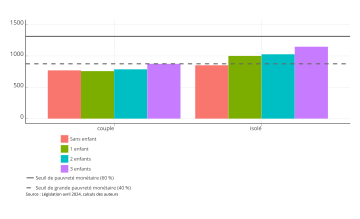
\includegraphics[keepaspectratio]{PB_GainEmploi_files/figure-pdf/fig-ndvminimum-1.png}}

}

\end{figure}%

Le niveau de vie des ménages sans revenus d'activité est faible. Il a
décru dans le temps et relativement aux autres revenus. Depuis 1990, le
niveau du minimum social en direction des personnes d'âge actif a ainsi
progressé bien moins vite que le niveau du minimum vieillesse (ASPA) ou
de l'allocation adulte handicapée (AAH) (graphique).

En 1989, la loi instaurant le RMI a pour principal objectif de donner un
minimum social pour les personnes valides d'âge actif. Si l'objectif est
principalement distributif, le législateur a néanmoins voulu préserver
les incitations à travailler en fixant le niveau du RMI à 50 \% du SMIC
à temps plein (mais en l'indexant sur l'inflation et non pas sur le
niveau du Smic ou du SMPT). Les débats font alors apparaître la volonté
de garder une norme d'emploi à plein-temps. Dans les années 1990, le
nombre d'allocataires augmente rapidement et atteint un niveau non
anticipé par les décideurs publics : de 500~000 allocataires en 1990, ce
nombre dépasse le million en 1996. Face à cette montée rapide, le
discours sur les « trappes à pauvreté » se répand. En 2001,
l'introduction de la prime pour l'emploi (PPE) est une première réponse
à ce discours. La PPE étant accusée d'être mal ciblée et de pénaliser
les emplois à temps partiel, le RSA activité prend la relève en 2009 et
permet de garantir que le revenu disponible d'un foyer augmente lorsque
ses revenus d'activité augmentent, même à temps partiel ou très partiel.
Il est ensuite remplacé par la prime d'activité en 2015, revalorisée
lors de la crise des gilets jaunes pour les salaires proches du Smic.
Durant cette période d'attention aux gains à l'emploi et à la pauvreté
laborieuse, le montant de base du RSA est peu revalorisé. Quelque part,
le dilemme entre incitation monétaire et redistribution est indépassable
: incitation et inégalités sont les deux face de la même pièce.

Pourtant, malgré l'augmentation des gains à la reprise d'emploi via le
creusement de l'écart entre le RSA et le SMIC et la montée en charge des
compléments de revenus pour travailleurs pauvres, la part d'allocataires
du RSA dans la population d'âge actif a augmenté, passant de 3,0\% en
2008 à 4,1\% en 2022. La réduction du niveau de vie relatif du RSA n'a
donc pas eu d'effets visibles en termes de baisse du nombre
d'allocataires.

\begin{figure}[H]

\caption{\label{fig-minimasociaux}Evolution des mimina sociaux et du
Smic horaire, base 100 = 1990}

\centering{

\pandocbounded{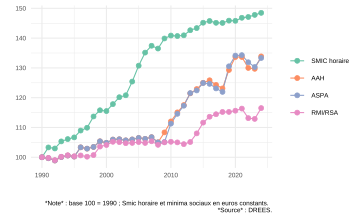
\includegraphics[keepaspectratio]{PB_GainEmploi_files/figure-pdf/fig-minimasociaux-1.png}}

}

\end{figure}%

\section{4. Peut-on dépasser les dilemmes du système social
?}\label{peut-on-duxe9passer-les-dilemmes-du-systuxe8me-social}

Comme nous l'avons montré dans les sections précédentes, le système
social et fiscal remplit bien l'objectif qui lui a été fixé depuis la
mise en place du RSA en 2009 : rendre le travail plus rémunérateur que
l'assistance. Mais avoir un emploi rémunéré au Smic n'est pas un gage de
sortie de la pauvreté, et vivre sans emploi implique souvent d'être dans
une situation de grande pauvreté. Le système ne remplit donc pas les
objectifs fixés par la SNPLP. Est-il possible d'y parvenir en modifiant
les barèmes du RSA et de la prime d'activité~? Nous explorons ici les
effets potentiels d'une hausse du socle (RSA et forfait de PA) ou d'un
ciblage de la prime d'activité sur le temps partiel et discutons des
limites d'un soutien aux bas salaires par une hausse du Smic ou de la
prime d'activité.

\subsection{4.1 Avantages et limites d'une augmentation du
socle}\label{avantages-et-limites-dune-augmentation-du-socle}

Il est possible de concilier les trois objectifs - travail rémunérateur,
travail permettant de sortir de la pauvreté et niveau de vie minimum
suffisamment élevé - en relevant le montant des prestations de
solidarité (RSA et aides au logement) et en gardant un minimum
d'incitations. En effet, si les personnes en emploi restent pauvres
malgré les allocations et les incitations\ldots{} c'est qu'ils partent
de trop bas. Le socle RSA pourrait être revalorisés de telle sorte qu'un
foyer sans emploi atteigne 50 \% du niveau de vie médian, soit 1 090
euros pour une personne isolée sans enfant, et 2 290 euros pour un
couple avec deux enfants. Avec les aides au logement actuelles, pour la
personne seule vivant en zone 2 (villes de plus de 100 000 habitants),
cela amènerait le montant du RSA et le forfait de prime d'activité avant
forfait logement à 900 euros. On peut alors maintenir le niveau des
points de sortie de la prime d'activité avec un taux de cumul de 45\%
(au lieu de 61\%). Cette revalorisation du socle permettrait aux couples
avec deux enfants de franchir le seuil de pauvreté monétaire avec un
seul emploi au Smic à temps plein.

Cette réforme est celle qui permettrait d'atteindre les trois objectifs
à la fois de manière cohérente. Elle est également la plus juste dans la
mesure où elle réduit fortement les inégalités avec, probablement, de
très faibles coûts en termes d'efficacité et d'emploi (voir par exemple
Bargain, 2014 et Simmonet et Danzin, 2014).

Mais cette réforme est aussi la plus coûteuse. Comme le montre notre
simulation (voir encadré) augmenter le socle à 900 euros avec une légère
baisse du taux de cumul de la prime d'activité aurait un coût d'environ
24 milliards d'euros pour les pouvoirs publics, dont 11 milliards de RSA
et 13 milliards de prime d'activité. Le dilemme entre redistribution et
incitation est en fait un triangle d'incompatibilité entre
redistribution, incitations monétaires et coût budgétaire (Bozio et
Grenet 2017).

Une solution permettant de réduire le coût serait de réduire bien plus
fortement le taux de cumul entre prestation d'assistance et revenus du
travail, de sorte que les bénéfices de la hausse soient ciblés sur les
plus pauvres. Nous avons simulé un scénario dans ce sens (taux de cumul
de 35\% de la prime d'activité au lieu de 45\%) qui présente
l'inconvénient majeur de faire des perdants très bas dans l'échelle de
revenus tout en réduisant drastiquement les gains à l'emploi.

On peut interpréter le coût de cette réforme comme une mesure de
l'injustice du système actuel même si cela n'implique pas que la réforme
proposée est la meilleure manière de dépenser cet argent pour améliorer
la situation des plus pauvres.

\begin{longtable}[]{@{}
  >{\raggedright\arraybackslash}p{(\linewidth - 0\tabcolsep) * \real{1.0004}}@{}}
\toprule\noalign{}
\endhead
\bottomrule\noalign{}
\endlastfoot
\textbf{Encadré : L'aide à sortir de l'assistance ne doit-elle concerner
que le travail?}

Le débat sur les gains, les taux de prélèvements, les incitations ne
concernent aujourd'hui que le travail. Cela montre l'importance du
«~mérite~» associé au travail dans ce débat public, indépendamment des
difficultés rencontrées par certains pour accéder à l'emploi. Les
pauvres peuvent cumuler (partiellement) leurs revenus du travail avec
leurs prestations sociales, mais ce n'est pas le cas des autres
ressources comme les revenus de remplacement (retraite, chômage), les
pensions alimentaires, les héritages et les dons, les gains aux jeux,
les loyers reçus pour un logement loué, la valeur locative des logements
non loués (!), les revenus des capitaux, et les revenus fictifs des
biens non productifs, comme les contrats d'assurance-vie, imputés à
hauteur de 3\% de leur valeur marchande. Or, nombre de ces ressources ne
sont pas comprises dans la base fiscale des plus aisés, le conseil
constitutionnel ayant même tranché contre la prise en compte de revenus
non effectifs (la valeur locative de logements non loués ne peut rentrer
dans le revenu au titre de l'imposition sur le revenu)\footnote{Pour les
  plus riches, grâce au prélèvement forfaitaire unique (PFU) le taux
  d'imposition est plus faible sur les revenus du capital que sur les
  revenus du travail.}. Mais le RSA, prestation d'assistance, ne suit
pas une logique de capacité contributive~mais une logique de
subsidiarité : le demandeur doit démontrer avoir fait valoir tous ses
droits, aux autres prestations sociales et créances alimentaires, et
même aux revenus de ses biens non utilisés. Tous les revenus non
professionnels sont déductibles à 100\% du RSA et de la prime d'activité
: un don de 100 euros, une chambre à louer, les revenus d'un peu
d'épargne. Cette logique crée des situations impossibles pour les
allocataires, mêmes sincères, s'ils reçoivent une aide familiale dans
une situation d'urgence, une chaudière qui tombe en panne, un enfant
malade, un évènement à l'autre bout de la France. Ils doivent déclarer
cette aide qui sera entièrement déduite de l'allocation versée. La
conséquence est qu'il y aura plus de fraudes détectées chez les
personnes vulnérables, obligées de contourner une technocratie d'autant
plus rigoureuse que cette rigueur est asymétrique entre les plus pauvres
et les plus aisés. C'est d'autant plus problématique que la rigueur du
calcul technocratique au moindre euro près s'applique à une prestation
faible. La situation décrite ici crée un phénomène de spirale de la
pauvreté puisque la moindre aide à s'en sortir, le moindre effort
d'épargne est annulé.

Une solution serait de rendre le calcul de la prestation davantage
bienveillant en mettant en place un abattement sur l'ensemble des petits
revenus (et non pas seulement les revenus du travail) : par exemple, les
450 premiers euros par trimestre (150 euros par mois) ne seraient pas
pris en compte dans le calcul de la prestation, quelle que soit leur
origine. Un autre avantage de cette solution est que le demandeur de
l'allocation ayant des petits revenus n'aurait pas à détailler leur
origine lors de la demande, il cocherait simplement la case « ressources
inférieures à 450 euros ». Un tel système réduirait la peur de se
tromper, la peur des indus à rembourser, et donc le non-recours. Les
premiers revenus d'activité seraient gardés à 100 \% par les
travailleurs, ce qui répond aussi à la problématique des coûts fixes à
la reprise d'emploi. Au-delà de l'abattement, le taux de cumul des
revenus d'activité et de la prime d'activité pourrait être abaissé pour
garder les gains à la reprise d'emploi à plein temps constants par
rapport à la situation actuelle. Si l'objectif est que les allocataires
des minima sociaux en sortent par le haut, il faut aussi éviter
d'annuler le moindre coup de pouce ou coup de chance. \\
\end{longtable}

\subsection{\texorpdfstring{4.2 \textbf{Soutenir les emplois à temps
partiel ou promouvoir la norme du temps
plein~?}}{4.2 Soutenir les emplois à temps partiel ou promouvoir la norme du temps plein~?}}\label{soutenir-les-emplois-uxe0-temps-partiel-ou-promouvoir-la-norme-du-temps-plein}

Faut-il cibler les compléments de revenus pour travailleurs au niveau du
temps-partiel ou du temps-plein ? Posé comme cela, le problème est
insoluble : pour protéger de la pauvreté, il vaut mieux inciter au
temps-plein ; mais pour réduire directement la pauvreté laborieuse, il
vaut mieux donner plus aux travailleurs à temps-partiel, qui ont des
niveaux de vie plus faibles, souvent sous le seuil de pauvreté. Le débat
sur la place du temps-partiel dans le dispositif de compléments de
revenus pour travailleurs à bas revenus, date des débuts de la prime
pour l'emploi en 2001 (voir notamment Cahuc, 2002). Redistribution et
incitation sont des objectifs non seulement inconciliables mais
contradictoires. La redistribution implique de réduire les écarts de
revenus disponibles entre non-emploi, temps partiel, temps-plein au Smic
et emploi mieux rémunéré. L'incitation implique de les maintenir ou de
les augmenter. Il est possible de dépasser le dilemme localement (en
augmentant le revenu disponible par les transferts à la fois à
temps-partiel et à temps-plein au Smic), mais le problème est alors
déplacé plus haut, à l'endroit où la prestation devient dégressive. On
parle aujourd'hui de trappes à bas salaires (voir le rapport
Bozio-Wasmer, 2024).

A la redistribution et l'incitation, s'ajoute un autre objectif :
rémunérer le «~mérite~». Il est probable que beaucoup d'acteurs ont cet
objectif en tête lorsqu'ils défendent l'idée que le travail doit payer
(Allègre, 2011). Mais dans cet optique, faut-il cibler la prime
d'activité sur le temps-partiel ou sur le temps-plein ? Tout dépend de
la norme sociale prédominante. Deux philosophies s'opposent. Selon la
première, le travail à temps-plein doit payer. Il faudrait créer une
norme de temps-plein, forme d'emploi la plus propice à réduire la
pauvreté. A la création du RMI, l'écart entre le RMI et le Smic a été
calculé sur la base d'un temps-plein. Initialement, le montant du RMI a
été fixé à 50\% du Smic. Cet écart peut être interprété en termes
incitatif ou de mérite. Selon la seconde philosophie, chaque heure de
travail doit payer, c'est-à-dire mérite une hausse du revenu disponible.
La volonté de créer un écart de revenus à la fois entre l'inactivité et
le mi-temps et entre le mi-temps et le temps-plein crée une pression à
la baisse sur le niveau des revenus d'assistance (et en haut la création
de ``trappes à bas salaires''). En 1989, la norme d'emploi était le CDI
à temps-plein. Le RMI était différentiel : après période d'intéressement
temporaire\hyperref[_ftn2]{{[}2{]}}, chaque euro de revenus
supplémentaires se déduisait à 100\% du revenu versé. Cela veut dire
qu'à terme une personne seule reprenant un emploi à mi-temps n'avait
aucun gain financier par rapport au revenu d'assistance. Les gains
étaient concentrés entre le mi-temps et le temps-plein. À cette époque,
malgré l'absence de gain financier, il y avait tout de même des reprises
d'emploi à temps partiel et même du cumul assistance-emploi (Guillemot,
Petour et Zajdela, 2002), signe que les personnes concernées
reconnaissaient les aspects positifs de l'emploi au-delà du revenu.
Faut-il revenir à une prestation différentielle pour augmenter le socle
? Une possibilité est de revenir au système prévalent de 1989 jusqu'à la
création du RSA en 2009. Ce système permet à la fois d'avoir un socle
plus élevé et de réaffirmer le temps-plein comme norme de travail et de
renforcer cette norme non pas avec des mesures qui visent les
travailleurs, mais en visant les entreprises et en limitant le nombre de
postes à pourvoir à temps-partiel (voir conclusion).

\subsection{\texorpdfstring{4.3 \textbf{Augmenter les gains à l'emploi
par la hausse du Smic ou grâce à la prime d'activité
?}}{4.3 Augmenter les gains à l'emploi par la hausse du Smic ou grâce à la prime d'activité ?}}\label{augmenter-les-gains-uxe0-lemploi-par-la-hausse-du-smic-ou-gruxe2ce-uxe0-la-prime-dactivituxe9}

Faut-il privilégier le soutien aux bas-salaires via le Smic (les
salaires) ou via la prime d'activité et ses bonus individuels renforcés
à la suite de la crise des gilets jaunes ? Smic et prime d'activité ne
sont pas équivalents car la prime d'activité n'est pas un salaire :

--- Le salaire est totalement individualisé : le bénéfice de la prime
pour un travailleur à bas salaire dépend de la composition de sa
famille, du montant et de la nature des revenus de son conjoint

--- Le salaire est plus prévisible pour les travailleurs. Ils peuvent
difficilement anticiper le montant de la prime d'activité compte tenu de
son mode de calcul et des risques d'indus et de suspension/rappels

--- le salaire procure des droits sociaux : le taux de remplacement au
chômage ou à la retraite est réduit pour les bénéficiaires de la prime
si l'on raisonne en revenus nets.

Avec le système actuel, les pouvoirs publics poursuivent deux
objectifs~: lutter contre la pauvreté et augmenter les gains à l'emploi
dans une logique de mérite. Or pauvreté et niveaux de vie sont par
construction familialisés tandis que le salaire et le mérite sont par
construction individuels (Ponthieux, 2009). L'hybridation de ces deux
logiques, la lutte contre la ``pauvreté laborieuse'', crée des
situations paradoxales. Par exemple, dans le système actuel, si dans un
couple biactif l'un des conjoints perd son emploi et touche des
allocations chômage, alors cela entraine la perte de la prime d'activité
pour le couple car les allocations chômage sont intégralement déduites
du revenu garanti du foyer. La perte d'emploi annule ainsi le droit à la
prime du conjoint mais aussi les éléments de primes liés à la charge
d'enfants. Le paradoxe est le suivant : si l'on donne un poids à
l'objectif de réduction de la pauvreté laborieuse, au-delà de celui que
l'on donne à l'objectif de réduction de la pauvreté, alors il est
préférable que certains pauvres ne travaillent pas. Résoudre le paradoxe
nécessite de démêler les vrais objectifs afin de les rendre cohérents.
Les objectifs sont les suivants. Premièrement réduire la pauvreté et les
inégalités de niveau de vie. Deuxièmement, augmenter l'emploi pour
réduire le coût public de la pauvreté. C'est alors un objectif
budgétaire, et non un objectif paternaliste selon lequel l'emploi serait
toujours bon pour les personnes concernées. Dans une logique
non-paternaliste, si le fait d'être en emploi est bon pour les
bénéficiaires des allocations, il n'y a pas de raison qu'ils ne le
reconnaissent pas et qu'ils aient besoin d'incitations pour travailler.
Lorsqu'il n'y avait pas de gain monétaire à cumuler RMI et faibles
heures de travail, de nombreux allocataires le faisaient tout de même.

Selon le principe de Tinbergen, lorsqu'il y a deux objectifs distincts,
ici la lutte contre la pauvreté et les gains à l'emploi, il faut
affecter à des instruments distincts la poursuite de ces objectifs. Dans
cette optique, on pourrait considérer que le RSA et une prime d'activité
entièrement familialisée (sans bonus individuels) permettent de lutter
contre la pauvreté et les inégalités de niveau de vie mais n'ont pas
pour objectif d'augmenter les gains l'emploi. Dans ce cas, il faudrait
étendre le bénéfice de la prime d'activité aux chômeurs (les
travailleurs sans emploi). Pour ce qui est de l'objectif de soutien aux
bas salaires, le Smic, associé à la norme du temps plein, doit être
l'instrument monétaire privilégié. Si l'objectif est la lutte efficiente
contre la pauvreté, alors il faut éviter que les entreprises puissent se
reposer sur le système social pour proposer des emplois qui ne seraient
pas viables par ailleurs.

\begin{longtable}[]{@{}
  >{\raggedright\arraybackslash}p{(\linewidth - 0\tabcolsep) * \real{1.0003}}@{}}
\toprule\noalign{}
\endhead
\bottomrule\noalign{}
\endlastfoot
\textbf{Encadré : simulation de deux réformes : quelques ordres de
grandeur}

Nous simulons deux réformes illustratives pour donner des ordres de
grandeur concernant le coût de ce types de réformes ainsi que la
répartition des foyers gagnants ou perdants. Pour cela, nous utilisons
le modèle de microsimulation sociale et fiscale INES développé par
l'INSEE, la DREES et la CNAF. La version utilisée d'INES simule la
législation 2022 sur les données de l'Enquête Revenus fiscaux et sociaux
(ERFS) 2020 actualisées à l'aide des dernières données démographiques et
économiques disponibles. Nos simulations font l'hypothèse d'un taux de
non-recours inchangé (en masse financière)\footnote{Dès l'instauration
  du RMI, un mécanisme d'intéressement a été mis en place, permettant le
  cumul temporaire des revenus d'assistance et des revenus du travail.
  Cet ``intéressement'' devait servir de marchepied vers l'emploi stable
  à plein-temps. Comme l'insertion professionnelle des bénéficiaires du
  RMI était jugée insatisfaisante, ce mécanisme fut réformé presque
  constamment. Entre 1989 et 1999, la prime d'intéressement était
  proportionnelle au salaire perçu lors des 750 premières heures
  d'emploi. Ensuite jusqu'en 2006, la prime était proportionnelle lors
  des 15 premiers mois de reprise. Puis jusqu'en 2009, la prime était
  forfaitaire pendant 9 mois, après 3 mois de cumul intégral.}. Les deux
réformes simulées s'appuient sur les points évoqués dans la section
précédentes. La première réforme consiste simplement à augmenter le
socle du RSA et à baisser le taux de cumul de la prime d'activité. Cela
répond directement au point 4.1. Une telle réforme serait moins
favorable aux incitations à temps-partiel (les travailleurs à
temps-partiel ne seraient pas perdants mais l'écart avec les revenus
d'assistance seraient réduits). Cette réforme est justifiée si on prend
au sérieux la lutte contre la grande pauvreté, si on souhaite verser un
revenu minimum un peu plus décent, et/ou si l'on considère que les
incitations ne jouent pas ou peu à ce niveau-là, les obstacles à la
reprise d'emploi étant autres que les faibles gains. Le problème de
cette réforme est son coût. Fixer le socle à 900 euros par mois pour une
personne seule, permettant d'atteindre le seuil de pauvreté à 50\%,
compensé par une baisse du cumul de la prime d'activité de 61 à 45\%
(qui laisserait le point de sortie de la prime d'activité constant pour
une personne seule) coûterait jusqu'à 30 milliards d'euros en plein
recours et 24 milliards d'euros à taux de recours inchangé. Par
construction, une telle réforme ne ferait presque pas de perdants :
presque tous les bénéficiaires du RSA et de la prime d'activité actuels
seraient gagnants mais il n'y aurait pas de gagnants au-delà. D'ailleurs
le coût en termes de prime d'activité (13 milliards à recours inchangé)
serait supérieur à celui du RSA (11 milliards). Par construction les
plus gros gains sont concentrés sur le premier décile (avec une
variation moyenne de revenu de 260 euros mensuels) puis sont très
fortement dégressifs (170 euros pour les foyers du 2ème décile des
niveaux de vie, et 60 € pour un niveau de vie médian). La deuxième
réforme consiste à changer le mécanisme de cumul. Afin de permettre aux
foyers allocataires de bénéficier de coups de pouces et de simplifier
les déclarations, nous permettons un cumul à 100\% jusqu'à 150 euros par
mois (en pratique 450 € par trimestre) de l'ensemble des revenus hors
prestations familiales et sociales (salaires, revenus de remplacement -
chômage, retraites, dons, revenus du patrimoine financier et foncier).
Le mécanisme se rapprocherait des mécanismes d'\emph{earnings
disregards,} relativement communs dans les pays anglo-saxons.
L'abattement de revenus peut être justifié par des coûts fixes de
reprise d'emploi ou pour minimiser les démarches administratives pour
des revenus très faibles. En gardant la même pente de prime d'activité,
le coût pour les finances publiques serait de 2,2 milliards en plein
recours et 1,8 milliard à taux de non-recours inchangé. Pour atteindre
la neutralité budgétaire, il conviendrait de réduire le taux de cumul de
la prime d'activité de 61 à 58,5\%. Cette réforme ferait quelques
gagnants en bas de l'échelle des revenus (9\% des ménages sont gagnants)
et des perdants au-delà (16\% de ménages perdants). Selon notre
microsimulation, les gagnants se situeraient surtout dans le 1er décile
(gain moyen de 19 euros mensuels sur l'ensemble des ménages du 1er
décile), tandis que les perdants se situent dans le 4ème décile (perte
de 8 euros mensuels). \\
\end{longtable}

\section{Conclusion : dépasser les dilemmes par la redistribution
réglementaire
?}\label{conclusion-duxe9passer-les-dilemmes-par-la-redistribution-ruxe9glementaire}

La réforme consistant à augmenter le socle nous parait la plus juste
dans la mesure où elle réduit fortement les inégalités, avec
-probablement- de très faibles coûts en termes d'efficacité et d'emploi.
Le problème principal d'une telle réforme est son coût, 24 milliards
d'euros à recours inchangé. On peut considérer que ce que montant est le
coût de l'injustice du système actuel tout en reconnaissant qu'il
pourrait être possible de faire mieux pour la population concernée avec
le même budget, autrement qu'avec ces prestations. Il existe en effet
une autre solution permettant de dépasser les dilemmes monétaires
exposés dans ce document. On peut parler de redistribution réglementaire
ou de redistribution des droits. De même que l'augmentation du Smic est
potentiellement peu ou pas coûteuse, jusqu'à un certain niveau, en
termes de finances publiques, c'est également le cas du renforcement des
droits des travailleurs les plus précaires, par exemple en renforçant le
droit au passage au temps-plein ou en pénalisant la fragmentation
journalière du travail. Devetter, Pucci et Valentin (2020) montrent que
le Smic n'est pas une protection suffisante contre la pauvreté des
travailleurs, du fait du temps partiel contraint dans des métiers dont
le taux horaire est faible. Le seuil de bas salaire mensuel (défini à
60\% du salaire médian) étant proche du Smic mensuel, par construction
les bas salaires manquent d'heures dans le mois par rapport à un
temps-plein. Les métiers les plus touchés par les bas salaires sont les
métiers du care, assistantes maternelles, aides à domicile (66\% de bas
salaires), les métiers du nettoyage (47\%), les métiers de
l'hôtellerie-restauration (50\%). Ces trois secteurs concentrent 43\%
des bas-salaires mensuels. Or ces professions concentrent forte
amplitude et faible densité de la journée de travail. Une réglementation
plus protectrice permettrait de réduire le recours au temps-partiel, ce
qui pourrait même limiter les besoins en termes de prime d'activité. Le
coût serait reporté sur les consommateurs de ces services. Le service de
nettoyage, l'aide aux personnes et la restauration n'étant pas
délocalisables, les risques sur l'emploi seraient limités.




\end{document}
